\section{Classification}
\label{sec:classify}

This work builds up on \cite{residual} that proposes combining the transformation that registers a template to a subject with the residual image that remains after the registration to construct a complete (lossless) image descriptor. The combined descriptor captures the group differences much better than their individual components, and it is more robust to varying registration accuracies. Since, the 4D transformation cannot capture all the details of the difference between the subject and the template, we use the residual to provide the additional information. This can be seen in Figure \ref{fig:def4d} where the transformation was unable to capture all the differences, specifically the wall thickening. The residual however captures that information accurately and therefore provides valuable information in addition to that provided by the 4D transformation.

As described in Section \ref{sec:4dreg}, we register the subjects to the template and estimate a 4-$D$ diffeomorphic transformation. This transformation, $H(\bx, t)$, is used to individually characterize the difference between the subject and the template, both anatomically and functionally. In other words, these deformations allow us to quantify and analyze how a group of subjects (say {\em healthy}) differ from another (say {\em diseased}). Since we estimate the transformation, we have the result of the warping as,
\begin{equation}
S(H(\bx, t)) = T(\bx, t) + D(\bx, t), ~~~~\forall (\bx,t) \in \Omega_T
\end{equation}
where $D(\bx, t)$ is the residual. 

Typically, myocardial tissue volumes, their volumetric changes, and the deformations obtained from the transformation are contrasted across individuals and groups in order to identify cardiomyopathic characteristics. The determinant of the Jacobian matrix of the displacement field at any point provides us with an estimate of the local volumetric change. Specifically, if the determinant is less than $1$, it implies local contraction and if it is greater than $1$ it implies local expansion. Thus the transformation characterizes the local changes in the myocardial tissue. This basically means using the transformation as an image descriptor and basing the classification purely on them. This would be a reasonable assumption if the transformation was able to align the subject perfectly with the template. This however is not true in reality and the natural variability in the cardiac anatomy and beating patterns makes it virtually impossible to estimate a diffeomorphic transformation that can align the two perfectly. Therefore representing the subject using only the transformation is an incomplete description of the subject.

Similar to the work proposed by Kara\c{c}al{\i} \cite{residual}, we propose a use of an extended descriptor by incorporating the residual $D(\bx, t)$. This has the advantage that in addition to characterizing the functional differences and the anatomical correspondences, the information over regions where the anatomies differ will be encoded by the residual. Another advantage of using the extended descriptor is that it reduces the need for aggressive registrations. Usually when using deformations as image descriptors for classification, the deformations have to be as accurate as possible, so that all changes can be captured. However, since we solve a non-linear energy minimization to estimate the deformations, it can take a very long time to converge to the global minima. Pairing the deformations with the residuals allow for the the deformations to be less than perfect, with the confidence that whatever feature overlooked by the registration will be captured by the residual. The combined descriptor benefits from the residuals at the lower end of registration accuracies, and from the 4-$D$ transformations at higher levels of accuracy. This makes the combined descriptor more robust under varying levels of registration performance.

%\subsection {Methodology}

% Let us consider the simplest classification problem in a cardiac case. Let us consider a group $\{S_i\}$ of MR cine sequences, which have been labeled as being {\em healthy} or suffering from a specific cardiomyopathy ({\em diseased}). Consider the transformations $H_i(\bx, t) = H_{S_i \leftarrow T}(\bx, t)$ that align the template $T$ to each subject $S_i$, 
% \begin{equation}
% \label{eq:res}
% S_i(H_i(\bx, t)) = T(\bx, t) + D_i(\bx, t), ~~~~\forall (\bx,t) \in \Omega_T
% \end{equation}
% The general idea is to pair the deformations $H_i$ with the residuals $D_i$ to represent the $i$th subject in the analysis. The joint descriptor $(H_i, D_i)$ is a complete representation, since we can reconstruct the subject $S_i$ with the knowledge of the descriptor at any point in the analysis, and thus, there is no loss of information.
% 
% The completeness of the representation comes at the cost of uniqueness, since for any given transformation we can come up with a unique residual so that Equation (\ref{eq:res}) is satisfied. In other words we can think of all the pairs $(H_i, D_i)$ satisfying Equation (\ref{eq:res}) as forming an equivalence class of representations $\mathcal{C}_i$ whole elements preserve the original information in $S_i$. Thus the task of classifying subjects can now be restated as being able to identify these equivalence classes.
% 
% \begin{figure}
% 	\begin{center}
% 		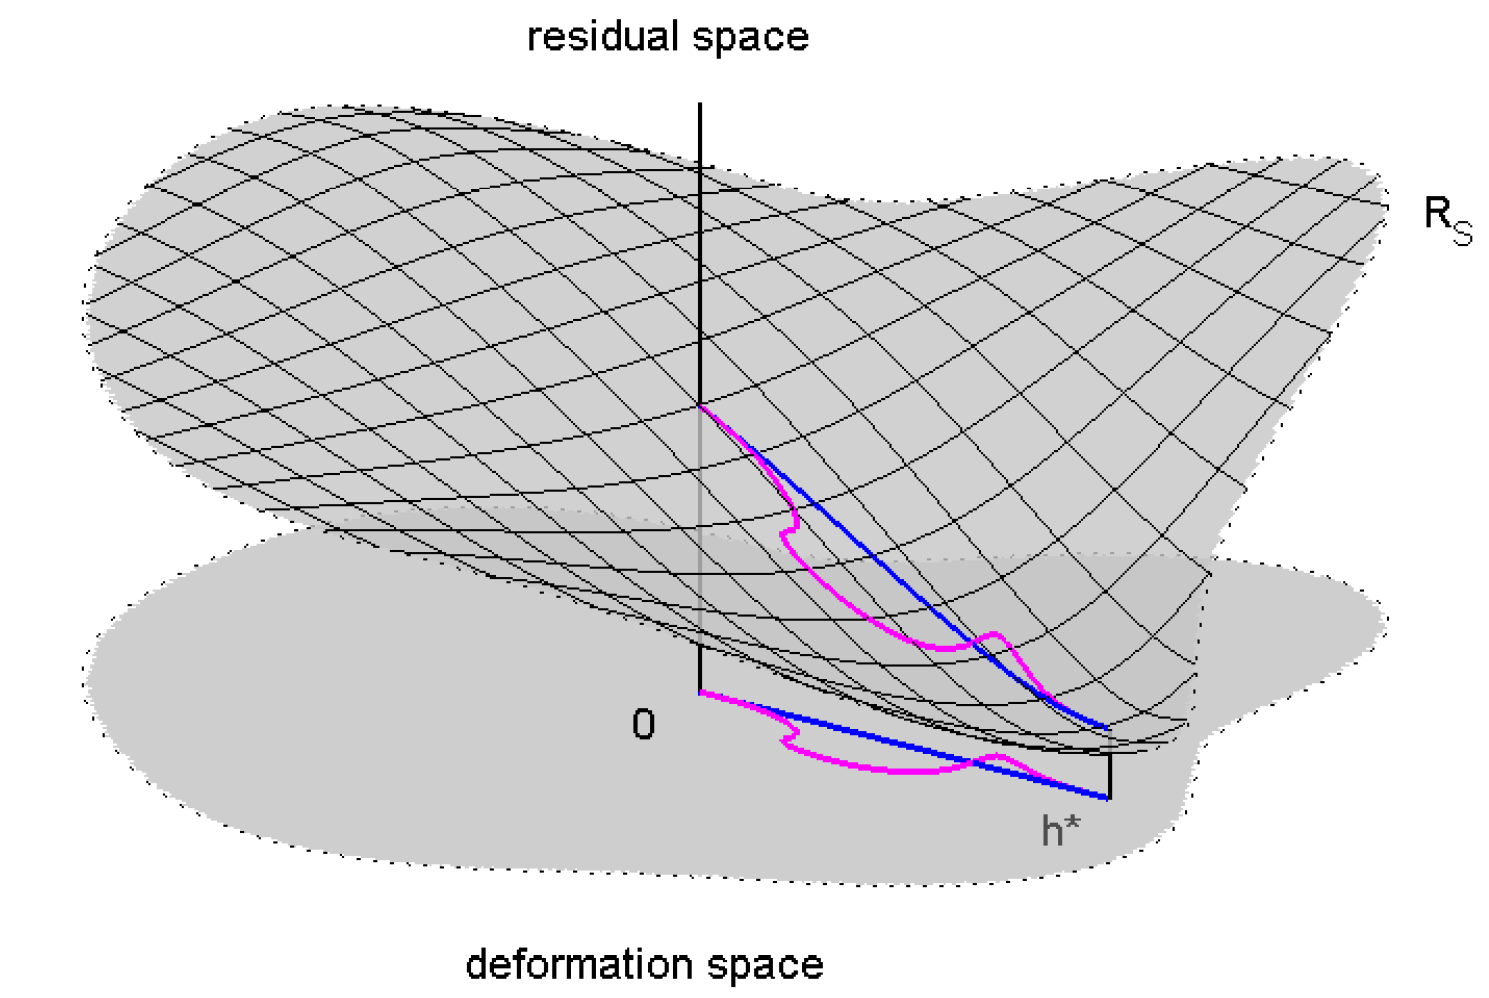
\includegraphics[width=.8\textwidth]{images/res_space}
% 	\end{center}
% 	\caption{Illustration of the equivalence class of representations}
% 	\label{fig:res_space}
% \end{figure}
% 
% This notion of equivalence classes for the transformation and residual pairs is illustrated
% in Figure \ref{fig:res_space}. The meshed surface represents the equivalence class of joint representations
% that satisfy Equation (\ref{eq:res}) for a given subject in the joint space of transformations
% and residual images specific to a given template. The template itself is situated at the
% origin, since in this space, it represents no residual to itself at zero deformation. A certain
% iterative registration algorithm produces the pink curve inside the equivalence class
% as it warps the template to the subject, and presumably achieves a relatively small residual
% $D_i$ for the deformation . The deformation estimates obtained by gradually smoothing
% the deformation $H_i$ and the corresponding residuals produce a more structured curve in the
% equivalence class illustrated by the blue line. A second subject would produce another equivalence class of representations represented by a different residual surface in this joint space of warping transformations and residuals. 
% 
% The equivalence classes of representations of all subjects correspond to similar but different
% hypersurfaces in the joint transformation-residual space. Consequently, comparing two
% subjects in terms of their equivalence classes of representations involves evaluating these two
% hypersurfaces through the continuum of transformations and corresponding residuals. Note
% that the hyper-surface illustration of these equivalence classes suggests that the residuals can
% be visualized as functions of the transformations, since given a warping transformation, there
% is a unique residual that satisfies Equation (\ref{eq:res}). We can therefore represent an equivalence
% class of joint representations as a graph of the residual function $R_S$ for a given subject $S$
% defined as
% \begin{equation}
% D = R_S(H)\stackrel{\Delta}{=} \mathcal{N}_{H}(S) - T
% \end{equation}
% where $\mathcal{N}_{H}(S)$ is the spatio-temporal normalization of the subject $S$ onto the template $T$ using the deformation $H$, i.e., $\mathcal{N}_{H}(S)(\bx,t) = S(H(\bx,t))$. The equivalence class $\mathcal{C}(S)$ of representations for the subject $S$ then becomes the graph $\mathcal{G}(R_S)$ of the residual function $R_S$,
% \begin{equation}
% \mathcal{C}(S) = \mathcal{G}(R_S) \stackrel{\Delta}{=} {(H, D)|D = R_S(H)}
% \end{equation}
% 
% In theory, the difference between the respective equivalence classes of representations of two
% subjects $S_i$ and $S_j$ can be measured using various metrics from functional analysis such as
% \begin{equation}
% \rho(R_{S_i}, R_{S_j}) = \left( \int_{H} \left\| R_{S_i}(H_i) - R_{S_j}(H_j) \right\|^2 dH \right)^{1/2}
% \end{equation}
% using a suitable norm on the residuals. In reality, however, this integral cannot be carried
% out over the space of all warping transformations. This necessitates selecting meaningful
% subsets of these equivalence classes and using the elements of these subsets to evaluate their
% similarities and differences. In theory, it is also possible to quantify the similarity between the
% equivalence classes representing two subjects using the minimum distance between members
% of respective classes, computed according to some definition of distance in the joint space of
% warping transformations and the residuals. Though plausible in principle, this strategy is
% very difficult to follow: it entails solving an optimization problem to find the two members
% that minimize the chosen distance measure, which is very computationally intensive due
% to the high dimensionality of the data, and also potentially very difficult to solve to begin
% with due to many local minima originating from the complexity of the residual function
% with respect to warping transformations. Furthermore, there is an additional difficulty in
% generalizing this similarity measure to computing group statistics, primarily because it does
% not satisfy the triangle inequality required of conventional vector space distance functions.

% \subsection{Approach}

% Comparing equivalence classes of representations is possible only when they are identified
% with respect to a frame of reference, which we choose to be the dedicated template. Specifi-
% cally, we first perform a moderately aggressive registration for every image $S_i$ to the template
% $T$, and construct an equivalence subclass by considering the warping deformations obtained
% by smoothing the original deformation using wavelet shrinkage \cite{donoho95} and pairing them with
% the corresponding residuals.

% The rationale in obtaining smooth versions of the original deformation $H_{S \leftarrow T}$ by reducing the
% $\mathcal(l)_1$ norm comes from a series of optimality properties of wavelet shrinkage in regularization
% theory. The $\mathcal(l)_1$ norm of the wavelet transform of a signal has long been established as a
% measure of sparsity of the signal representation \cite{chen98}. The signal estimates obtained using
% wavelet shrinkage have been shown to achieve the optimal trade-off between the estimation
% error and the smoothness of the representation.

% These equivalence subclasses constructed by gradually smoothing a warping transformation
% that achieves a reasonably accurate registration between a given subject and a template.
% In that sense, they possess certain key properties as opposed to other possible collections
% of image descriptors. In particular, they represent the trade-off between the flexibility of
% the warping transformation and the magnitude of the residual over a continuum. The representation
% with most flexible transformation in the equivalence subclass is associated with
% the smallest residual not only in the equivalence subclass, but also for all transformations
% in a certain local neighborhood. At the other end of the equivalence subclass, the transformation
% is very smooth at the expense of a much larger residual. In addition, they yield
% themselves to comparison better than the full equivalence classes or their arbitrarily selected
% subsets for several reasons. First and foremost, they express similarity towards a common
% anatomy, namely, the chosen template. The $\mathcal(l)_1$ norms of the warping deformations, for instance,
% measure how much deformation the template needs to undergo in order to match
% the given subject. The subjects that are more similar to the template would presumably
% require smaller deformations to be spatially normalized to it. These deformations would
% also be characterized by small $\mathcal(l)_1$ norms, indicating the absence of strong warping components.
% When compared across individuals, smaller $\mathcal(l)_1$ norms in the high accuracy warping
% transformations are therefore indicative of subjects that are more similar to the template.

% Secondly, when the joint image descriptors are constructed from the warping deformations
% of all subjects which have the same $\mathcal(l)_1$ norm and their corresponding residuals, the
% regional distribution of the deformations and the residual energies indicate the morphological
% structures over which the subjects are similar and dissimilar to the template. The smaller
% $\mathcal(l)_1$ norm is a limited resource for registration, which is used optimally in the smooth estimate by the wavelet shrinkage. The spatial distribution of this resource over the brain would
% inevitably be different for different subjects in order to accommodate individual anatomical
% variability as best as possible. Patterns of this distribution would then reveal anatomical
% characteristics between individuals and their respective populations.
% Additionally, the fact that the flexibility of the deformations are limited equally for all
% subjects with a given $\mathcal(l)_1$ norm creates a platform suitable for comparing the image description
% pairs across individuals. A true comparison of subjects in terms of their original equivalence
% classes of representations entails a functional comparison of the residuals for all conceivable
% warping transformations. Since this cannot possibly be done over the continuum, a small
% collection of transformations are to be selected. On the other hand, not all transformation-residual
% pairs can be expected to be equally informative for all subjects. Selecting the joint
% descriptors that have the same $\mathcal(l)_1$ norm in their transformation components for all subjects
% puts individually tuned representations in the same context for comparison.
